\chapter{A Simple GUI for the Hybrid NLP Element}

This chapter introduces a Graphical User Interface (GUI) developed as part of 
this work in order to 
facilitate analyses using the hybrid \acrshort{nlp} element. We detail the 
various features that are implemented using the AppDesigner utility of MATLAB, 
version 2022b. The chapter is divided in seven sections, each representing a 
particular tab of the interface. These seven tabs are : 1) Mesh, 2) Materials, 
3) Sections, 4) Boundary Conditions, 5) Analysis Controls, 6) Solve Job and, 
finally, 7) Post-processing. The first five tabs, some of which can be edited 
independently, belong to the pre-processing phase. Tab 6 calls the hybrid NLP 
solver for the given input in tabs 1-5 and tab seven provides post-processing 
infrormation with respect to the structure response in the form of 
force-displacement plots and  configuration history for all steps. A number of 
tooltips can be revealed by hovering over relevant fields.

\section{The Mesh Tab}

The first tab of the GUI, depicted in Fig. \ref{fig:TAB1_marked}, is concerned 
with nodal and element input. We analyze it in terms of parts A to M:

\begin{itemize}
	\item \textbf{A}: The Mesh tab.
	\item \textbf{B}: Facility used to manually add nodes. Numeric values 
	pertaining to the X (horizontal) and Y (vertical) coordinate axes are used 
	in the corresponding fields to define the coordinates of a node. By 
	clicking on the \textit{Add Node} button, the enumerated node is added to 
	the table with its coordinated also listed. The enumeration is automatic. 
	Attempting to add a node with coordinates (X,Y) that are already defined 
	for another node results in an error, as shown in Fig. 
	\ref{fig:TAB1_node_error}.
	\item \textbf{C}: Facility used to delete a particular node. The 
	\textit{Label} field takes as input the node label already generated and 
	removes it from the table. The enumeration of remaining nodes is updated 
	accordingly. If node deletion is performed after the mesh is generated, the 
	latter is no longer valid and all elements are removed.
	\item \textbf{D}: Success/Error indicator of an action pertaining to node 
	generation, coupled with a text field for relevant message output (e.g. see 
	\ref{fig:TAB1_node_error}).
	\item \textbf{E}: Facility to generate a node set from a \textbf{.txt} or 
	\textbf{.xlsx} file. The format for this input file is shown in Fig. 
	\ref{fig:TAB1_nodesfile}. If a number of nodes have already been added 
	manually, this action replaces all existing nodes. In contrast, generating 
	a nodal set from an input file and then manually adding additional nodes 
	results in appending the previously generated nodal list.
	\item \textbf{F}: Table that lists all generated nodes along with their 
	coordinates.
	\item \textbf{G}: Facility used to manually add a (hybrid \acrshort{nlp}) 
	beam element. Since only one element per member is adquate with the 
	proposed formulation, the only relevant inputs are the start and end node 
	labels, indicated in the relevant fields as \textit{Node} $i$ and 
	\textit{Node} $j$ respectively. Again, adding an element with start and end 
	nodes already defined for an existing element results in an error. In 
	addition, element enumeration is, again, automatic.
	\item \textbf{H}: Element deletion facility. The element label used as 
	input in the relevant field and by clicking the \textit{Delete Element} 
	button results in removal of the particular element from the table. The 
	remainig elements are, again, automatically re-enumerated.
	\item \textbf{I}: Success/Error indicator of an action pertaining to 
	element generation, coupled with a text field for relevant message output.
	\item \textbf{J}: Facility to generate an element partition from a 
	\textbf{.txt} or \textbf{.xlsx} file. The format for this input file is 
	shown in Fig. \ref{fig:TAB1_elementsfile}. If a number of elements have 
	already been added manually, this action replaces all existing elements. In 
	contrast, generating an element partition from an input file and then 
	manually adding additional elements results in appending the previously 
	generated element list.
	\item \textbf{K}:  Table that lists all generated elements along with their 
	start and end nodes.
	\item \textbf{L}: Once clicked, the \textit{Clear Mesh} button resets all 
	existing input in the Mesh tab and the user can start over.
	\item \textbf{M}: GUI axes that dynamically update the existing state of 
	nodal and mesh configuration. Figure \ref{fig:TAB1_mesh_example} shows the 
	Mesh tab when the mesh generation is complete for a simple case of a one 
	bay, one story frame. The nodal labels are places right next to their 
	respective nodes and are typeset in normal font while element labels are 
	approximately placed in the midspan of their corresponding elements and are 
	typeset in italic bold fonts.
\end{itemize}

\begin{figure}
	\centering
	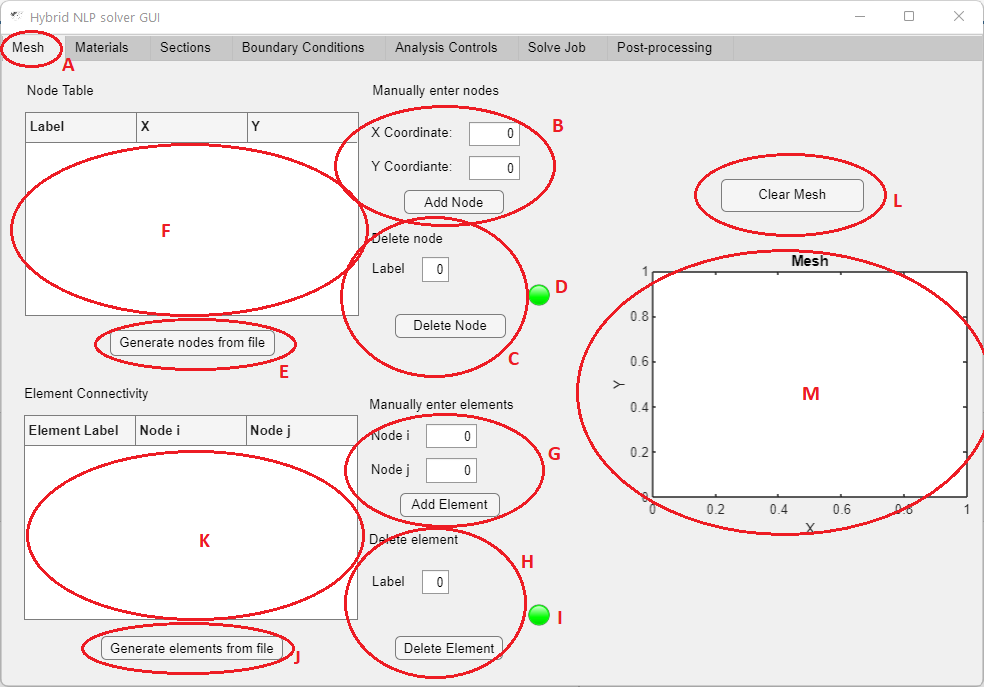
\includegraphics[scale=0.6]{GUIpics/TAB1/TAB1_marked.png}
	\caption{The Mesh tab with relevant facilities A-M marked in red circles 
	and enumerated with capital english letters.}
	\label{fig:TAB1_marked}
\end{figure}

\begin{figure}
	\centering
	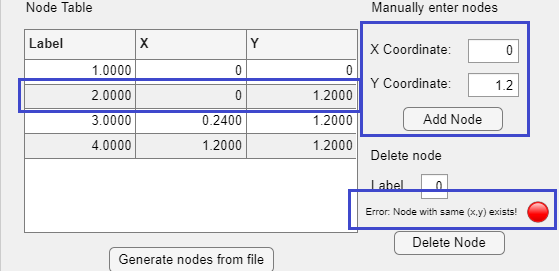
\includegraphics[scale=0.6]{GUIpics/TAB1/TAB1_node_error.png}
	\caption{Error when attempting to add a node with coordinates already 
	defined for an existing node.}
	\label{fig:TAB1_node_error}
\end{figure}

\begin{figure}
	\centering
	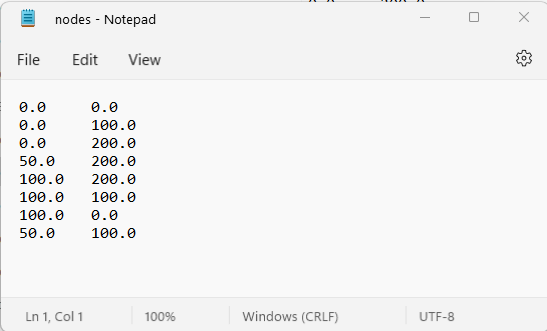
\includegraphics[scale=0.6]{GUIpics/TAB1/TAB1_nodesfile.png}
	\caption{A .txt file with the required format for nodal input. First column 
	is X coordinate, second is Y coordinate. The $k$-th row represents Node 
	$k$.}
	\label{fig:TAB1_nodesfile}
\end{figure}
\begin{figure}
	\centering
	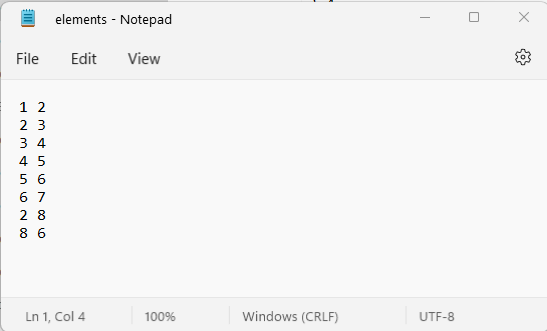
\includegraphics[scale=0.6]{GUIpics/TAB1/TAB1_elementsfile.png}
	\caption{A .txt file with the required format for element input. First 
	column is start node $i$, second is end node $j$. The $k$-th row represents 
	Element $k$.}
	\label{fig:TAB1_elementsfile}
\end{figure}

\begin{figure}
	\centering
	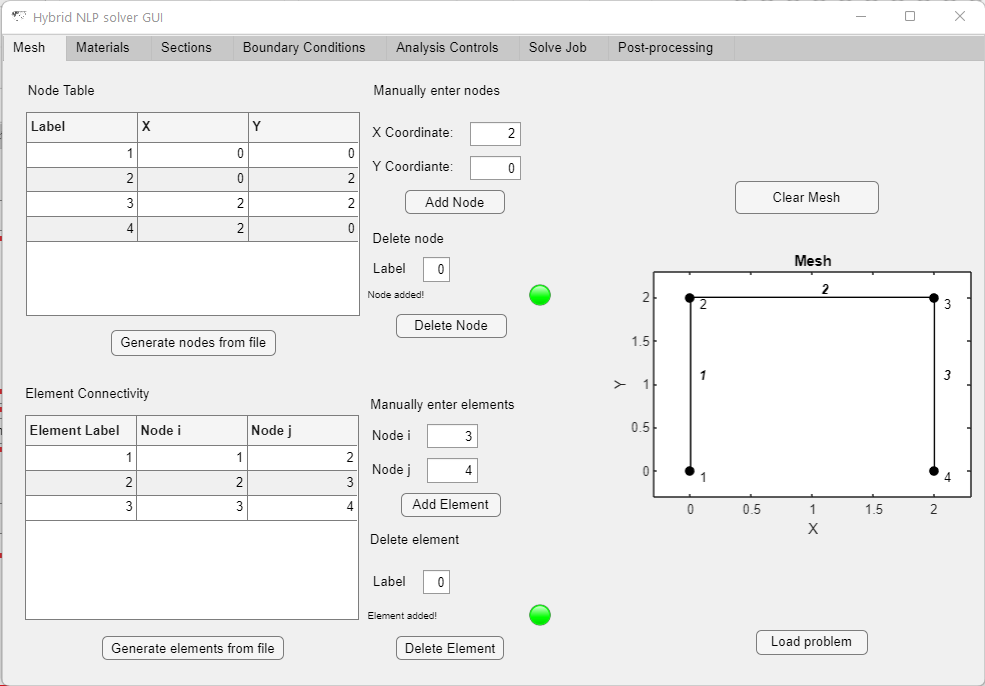
\includegraphics[scale=0.6]{GUIpics/TAB1/TAB1_mesh_example.png}
	\caption{The Mesh tab with a completed mesh.}
	\label{fig:TAB1_mesh_example}
\end{figure}


